\chapter{Data analysis framework}
\label{chap:artframework}

\section{Offline framework for the SLAC test beam}

\ac{midas} DAQ system is developed at \ac{psi} and \ac{truimf}.

\begin{figure}[htbp]
\centering
%\fbox{\includegraphics[trim=0cm 5.5cm 0cm 5.5cm ,width=0.9\textwidth]{pics/EMShower}} guide line for trimming
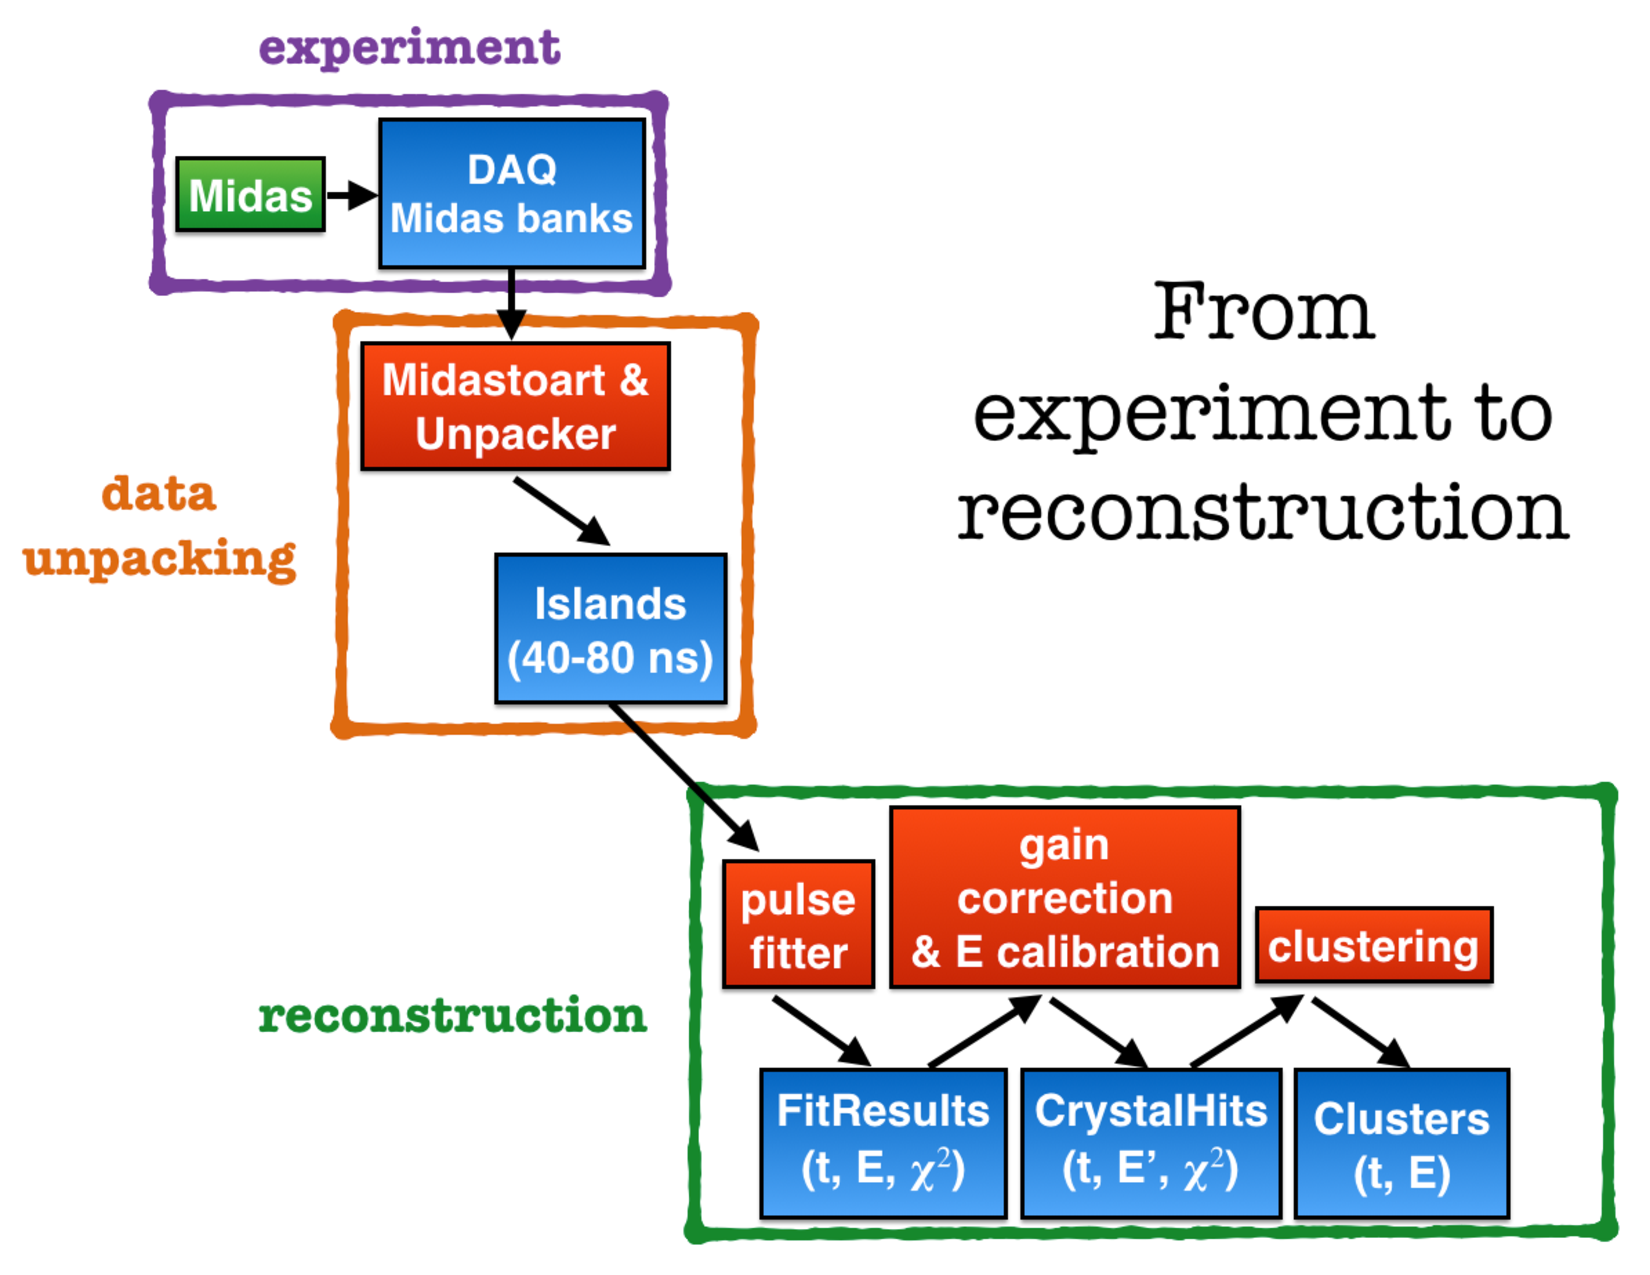
\includegraphics[width=0.7\textwidth]{pics/offline_exp_framework}
\caption{An overview of the Muon g-2 offline framework.}
\label{pic:exp_framework}
\end{figure}

As shown in \fref{pic:exp_framework}, data analysis for this test beam has several components. First we need to convert the raw data stored in a MIDAS file (\verb+.mid+ or \verb+.mid.gz+) to \textit{art} data products stored in an \textit{art} file.
This is handled using \textit{art} framework's modules and is doing nothing more than storing \verb+16-bit+ or \verb+32-bit+ word into \verb+vectors+. Next we unpack these \verb+vectors+
and give them contexts based on the header information stored within the \verb+vectors+. At this step, all the information are stored as data products you are probably familiar with: \verb+RiderArtRecord+,
\verb+IslandArtRecord+, etc. Then reconstruction algorithms are ran through these data products and at the end of the chain each physics objects are reconstructed as clusters.



\begin{figure}[htbp]
\centering
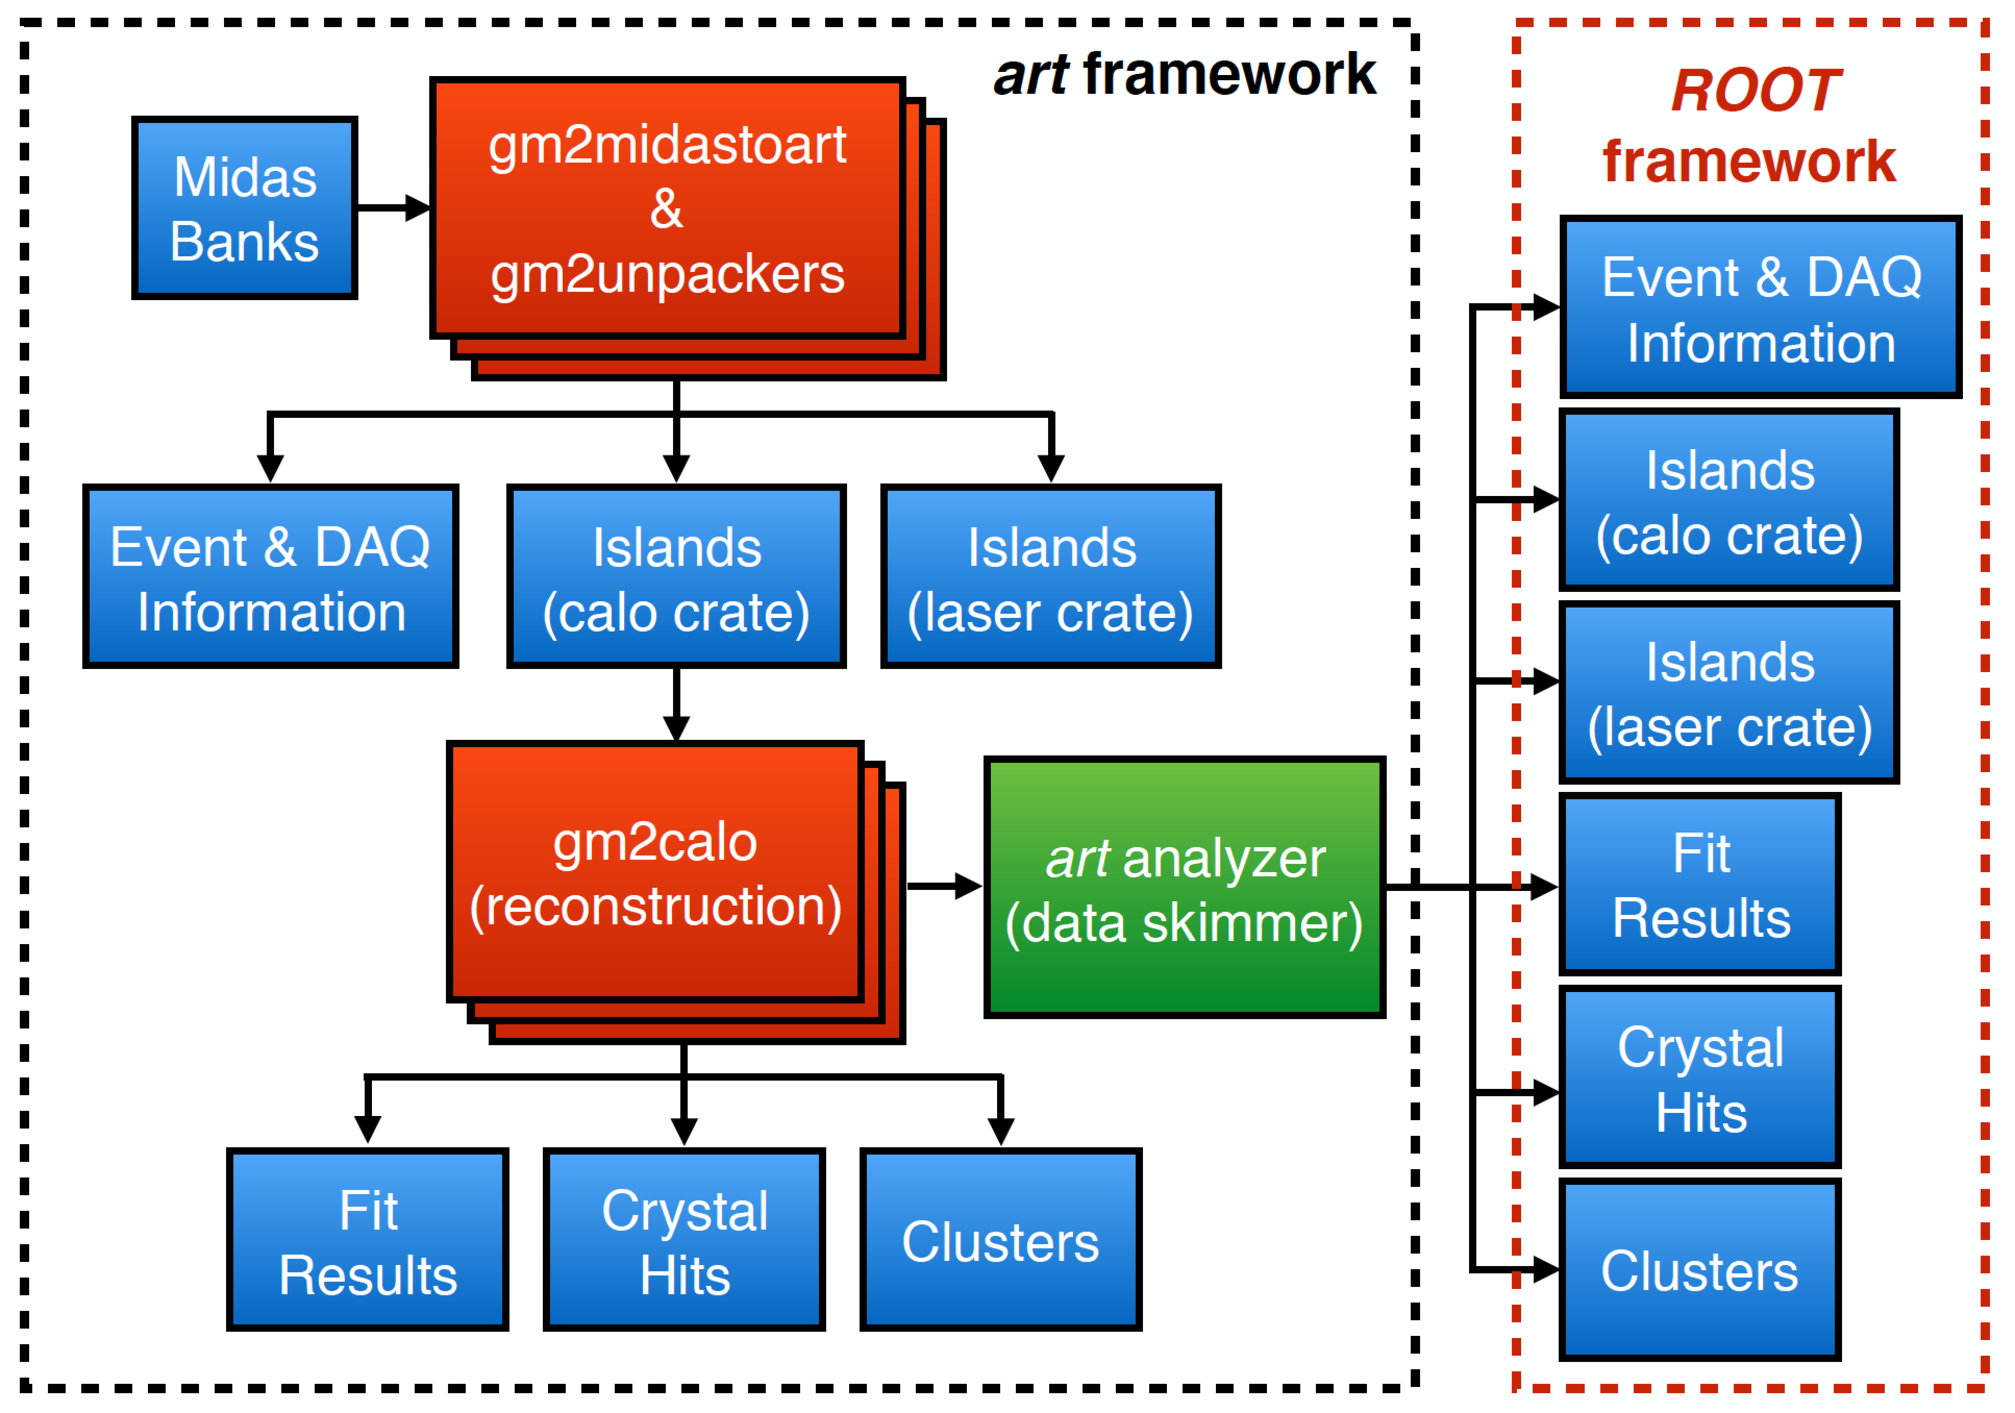
\includegraphics[width=0.7\textwidth]{pics/offline_slac_framework}
\caption{Offline framework for the SLAC experimental data.}
\end{figure}



